\chapter{STP}\label{sec:STP}

\section{Layer 2 loop}

Multiple cabled paths between switches provide physical redundancy. However, when  redundancy is introduced into a design, loops and duplicate frames occur. Loops and duplicate frames have severe consequences for network:

\begin{itemize}
\item Duplicate unicast frames
\item MAC database instability
\item Broadcast storm
\end{itemize}

\paragraph{MAC Database Instability:}Broadcast frames are forwarded out all switch ports, except the original ingress port. If there is more than one path to the destination, the frames may be forwarded back to the original switch, and create an endless loop. When a loop occurs, the MAC address table constantly changes with the updates from the broadcast frames, which results in MAC database instability. See this \href{https://ccnav6.com/s3/course/module2/2.1.1.2/2.1.1.2.html}{link} for more explanation.

\paragraph{Duplicate unicast frame:}MAC Database Instability makes the switch overwhelming and confused. It does not know destination MAC address and must forward the frame out all ports.  Consequently, unicast frames arrive at the destination device more than once.

\paragraph{Broadcast storm}occurs when there are so many broadcast frames caught in a Layer 2 loop. Consequently, all available bandwidth is consumed. No bandwidth is available for legitimate traffic and the network becomes unavailable for data communication. This is an effective denial of service (DoS). Broadcast storm also cause the end device to malfunction because of the processing requirements needed to sustain such a high traffic load on the NIC.

\section{STP overview}

\subsection{Operation}

The Spanning Tree Protocol (STP) was developed to prevent loops and duplicate frames. STP ensures that there is only one logical path between all destinations on the network by blocking redundant paths that could cause a loop. If failure occurs, STP recalculates the paths and unblocks the necessary ports to allow the redundant path to become active. Below are some options for STP:

\begin{itemize}
\item \textbf{802.1D} -- The first STP version, one spanning tree instance for the entire bridged network, regardless of the number of VLANs.
\item \textbf{PVST+} -- Cisco enhancement of STP, provide a separate spanning tree instance for each VLAN.
\item \textbf{RSTP or 802.1w} -- An standards-based evolution of STP.
\item \textbf{Rapid PVST+} -- Cisco enhancement of RSTP, provide a separate spanning tree instance for each VLAN.
\item \textbf{MSTP} -- Multiple Spanning Tree Protocol, an IEEE standard, map multiple VLANs into the same spanning tree instance. It can also ride on top of another spanning-tree protocol.
\item \textbf{MST} -- Cisco implementation of MSTP, provide up to 16 instances of RSTP.
\end{itemize}

\section{Bridge ID}

Bridge ID (BID) uniquely identifies a switch. The BID value is determined by the combination of three fields: \emph{bridge priority}, \emph{MAC address of the sending switch}, and \emph{extended system ID}. The \textbf{extended system ID} reserves the rightmost 12 bits for the VLAN ID and the far left 4 bits for the bridge priority. Therefore, the \textbf{bridge priority} value can only be the multiples of 4096 ($2^{12}$). If we consider BID as a hexadecimal number, the lowest left-most 4 bits (meaning lowest priority) always leads to lowest BID value.\\

\begin{figure}[hbtp]
\centering
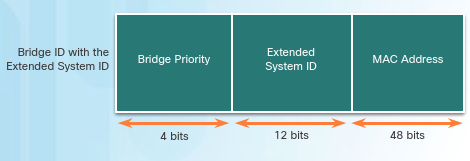
\includegraphics[width=0.6\textwidth]{pictures/BID.png}
\caption{BID fields}
\label{BID}
\end{figure}



\section{BPDU frame}

A Bridge Protocol Data Units (BPDU) is a frame exchanged by switches for STP. BPDUs have a destination MAC address of \textbf{01:80:C2:00:00:00}, which is a multicast address for the spanning tree group. A BPDU frame contains 12 distinct fields:

\begin{itemize}
\item The first four fields identify the protocol, version, message type, and status flags.
\item The next four fields are \textit{root ID}, \textit{bridge ID (BID)}, path cost.
\item The last four fields are all timer fields. They determine how frequently BPDU messages are sent and how long the information received through the BPDU process is retained.
\end{itemize}

\paragraph{Root ID} indicates the BID of the root bridge. When a switch first boots, the root ID is the same as the BID. However, as the election occurs, the lowest BID replaces the root ID to identify the root bridge.

\paragraph{Path cost}is the cost of the path from the sending switch to the root bridge. When a switch receives the BPDU, it adds the ingress port cost of the segment to determine its internal root path cost. The path cost is determined by summing up the individual port costs along the path from the switch to the root bridge. The default port costs are defined by the speed at which the port operates.

\tableStart[\caption{Default path cost}] {|l|l|}
\head{Port and speed} & \head{Cost} \w
10 Gb/s Ethernet & 2 \w
1 Gb/s Ethernet & 4 \w
100 Mb/s Ethernet & 19 \w
10 Mb/s Ethernet & 100\w
\tableEnd

\section{Root bridge election}

There is a root bridge elected for each spanning tree instance. The switch with the lowest priority is the root bridge. If the priorities are equal, then the switch with the lowest MAC address is elected the root bridge. All switches in the broadcast domain participate in the election process. After a switch boots, it begins to send out BPDU frames every two seconds. These BPDUs contain the switch BID and the root ID.\\

\begin{figure}[hbtp]
\caption{Root bridge selection}\label{RootBridge}
\centering
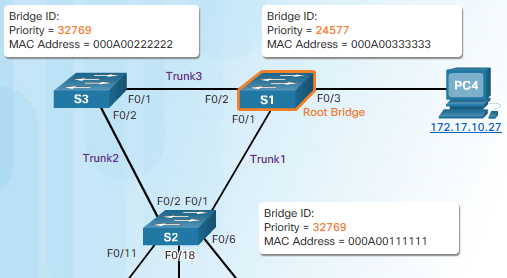
\includegraphics[ width=0.7\textwidth ]{pictures/RootBridge.PNG}
\end{figure}

Assuming that switch S1, S2, and S3 resides in the same broadcast domain (figure \ref{RootBridge}). As S1 forward a BPDU frame to S2, S2 reads the root ID from the BPDU frame, which is 24577-000A$\cdot$. Because the root ID from the BPDU frame is lower than the that of S2, which is 32769-000A$\cdot$, then S2 updates its root ID to 24577-000A$\cdot$. S2 then forwards BPDU frame with the newly updated root ID to S3. The same process repeats, S3 compares its current root ID with the root ID identified in the frames, and then updates its current root ID if needed. Eventually, the root ID of all switches equals 24577-000A$\cdot$ (the lowest BID). Therefore, all switches know exactly which one is the root bridge, based on the root ID. At this point, the election is complete.

\section{Port Roles}

\subsection{What is port role?}

Spanning Tree Algorithm (STA) determines which switch ports on a network must be blocked to prevent loops. It designates a single switch as the root bridge and uses it as the reference point for all path calculations (see figure \ref{STP-operation}). After the root bridge has been determined, STA assigns port roles to the switch ports:

\begin{itemize}
\item \textbf{Root port} -- Switch ports closest to the root bridge in terms of overall cost to the root bridge.
\item \textbf{Designated port} -- All non-root ports that are still permitted to forward traffic on the network.
\item \textbf{Alternate and backup ports} -- Alternate ports and backup ports are blocked to prevent loops. 
\end{itemize}

\begin{figure}[hbtp]
\centering
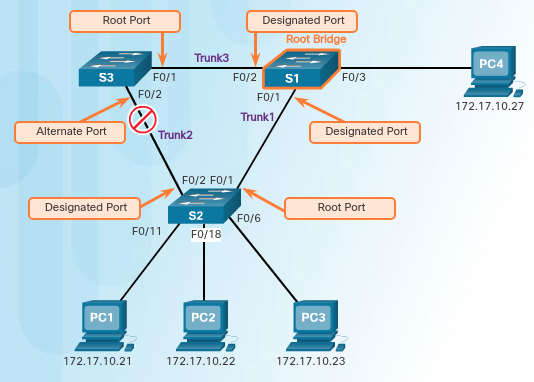
\includegraphics[width=0.8\textwidth]{pictures/STP-operation.png}
\caption{The STA designates a single switch as the root bridge}
\label{STP-operation}
\end{figure}

STA determines port roles on the following rules:

\begin{itemize}
\item There can only be one root port per non-root switch
\item If one end of a segment (the link between two switches) is a root port, then the other end is a designated port.
\item All ports on the root bridge are designated ports.
\item Alternate ports are elected only on segments where neither end is a root port.
\end{itemize}

After the root bridge is elected, the STA determines port roles (figure \ref{PortRole}) on the following steps in sequential order:

\begin{enumerate}
\item The root bridge automatically configures all of its switch ports in the designated role.
\item STP determines root port role. On each non-root switch, the port with lowest path cost to root bridge will become root port.
\item Non-root switches configure their non-root ports as designated or alternate ports.
\end{enumerate}

\begin{figure}[hbtp]
\caption{Port role assignment}\label{PortRole}
\centering
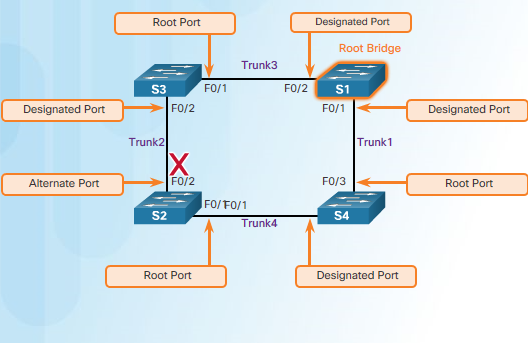
\includegraphics[ width=0.6\textwidth ]{pictures/PortRole.PNG}
\end{figure}


In the last step, two ports on the same segment will negotiate with each other. If one end of a segment is a root port, then the other end is a designated port. In figure \ref{PortRole}, the segment between S1(F0/1) and S2(F0/1) is an example.\\

However, when neither end of a segment cannot be a root port, the two switches on that segment exchange BPDU frames to decide which port to configure as a designated port. The switch with the lower path cost to the root bridge will have its port configured as a designated port. The other port will become an alternate port. If the path costs are equal, then the switch with the lower BID has its port configured as a designated port while the other has its port configured as an alternate port.\\

\begin{figure}[hbtp]
\caption{Redundant links}\label{Redundancy}
\centering
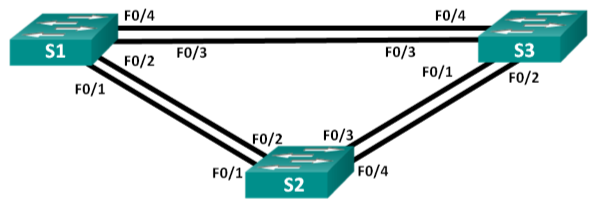
\includegraphics[ width=0.7\textwidth ]{pictures/Redundancy.PNG}
\end{figure}
 
If there are more than two paths in a segment (figure \ref{Redundancy}), then the port with the lower number (e.g. port number of F0/3 is lower than F0/4) will become active, while the other will be blocked.

\section{PVST+}

\subsection{Port state}

To facilitate the learning of the logical spanning tree, each switch port transitions through five possible port states:

\begin{itemize}
\item \textbf{Blocking:} The port is an alternate port and does not participate in frame forwarding. The port receives BPDU frames to determine the location and root ID of the root bridge switch and which port roles each switch port should assume in the final active STP topology.
\item \textbf{Listening:} The port is preparing to participate in frame forwarding. It listens for the path to the root. It also processes its own BPDU frames, and broadcast them to inform adjacent switches that the switch port is about to join the active topology.
\item \textbf{Learning:} The port learns the MAC addresses and populates the MAC address table. 
\item \textbf{Forwarding:} The port is considered part of the active topology. It forwards data frames and sends and receives BPDU frames. 
\item \textbf{Disabled:} The Layer 2 port does not participate in spanning tree and does not forward frames. The disabled state is set when the switch port is administratively disabled.
\end{itemize}

\begin{table}[h!]
\centering
\caption{Five port states in PVST+}
\label{PVST-port-state}
\begin{tabular}{|p{0.25\textwidth}|c|c|c|c|c|}
\hline

& \multicolumn{5}{c|}{Port states} \\ \hline
 
\head{Operation allowed}                           
& \head{Blocking} & \head{Listening} & \head{Learning} & \head{Forwarding} & \head{Disabled} \\ \hline

Receive BPDUs                                 
& *        & *         & *        & *          &        \\ \hline

Process BPDUs                                 
&          & *         & *        & *          &        \\ \hline

Learn MAC addresses                            
&          &           & *        & *          &        \\ \hline

Forward data frames           
&          &           &          & *          &        \\ \hline

\end{tabular}
\end{table}



\subsection{PortFast and BPDU guard}

When a switch port is configured with PortFast that port transitions from blocking to forwarding state immediately, bypassing the usual transition states (the listening and learning states). You can use PortFast on \emph{access ports}\footnote{Access ports are ports which are connected to an end device such as a PC or a server.} to help devices connect to the network immediately, rather than waiting for STP to converge on each VLAN. \\

\begin{figure}[hbtp]
\caption{PortFast and BPDU guard}
\centering
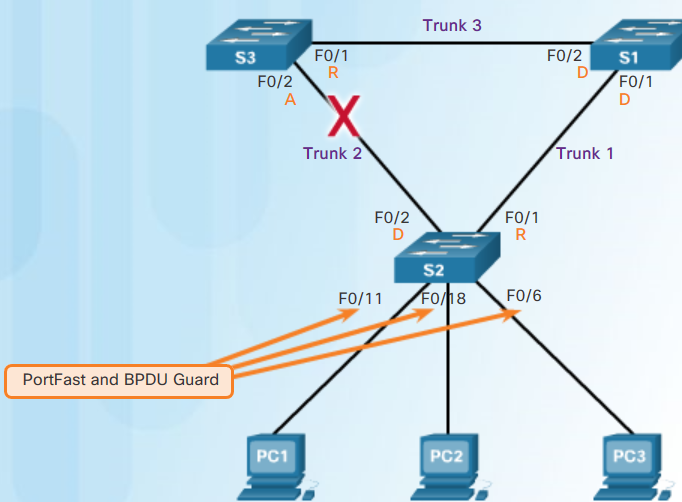
\includegraphics[ width=0.6\textwidth ]{pictures/PortFast.PNG}
\end{figure}

Because a PortFast-configured port is not connected to a switch, BPDUs should never be received. Otherwise, the broadcast domain will ``think'' that the port is connected to a switch. This consumption potentially causes layer 2 loops. To address this issue, Cisco switches support a feature called BPDU guard. This will effectively shut down the port. The BPDU guard feature provides a secure response to invalid configurations because you must manually put the interface back into service.\\

Cisco PortFast technology is useful for DHCP. Because PortFast immediately changes the state to forwarding, the PC always gets a usable IP address from DHCP server.


\section{RSTP and Rapid PVST+}

Rapid PVST+ is Cisco enhancement of RSTP. In this section, only the common features of these two protocols are discussed.

\paragraph{BPDU:} RSTP uses BPDU version 2, while 802.1D uses version 0. Protocol information can be immediately aged on a port if Hello packets are not received for three consecutive Hello times (six seconds, by default) or if the max age timer expires. BPDUs are used as a keepalive mechanism. Therefore, three consecutively missed BPDUs indicate lost connectivity between a bridge and its neighboring.\\

RSTP expands the STP port roles by adding the alternate and backup roles. It also combine blocking and listening port state to allow faster convergence. Port states are defined as \emph{discarding}, \emph{learning}, or \emph{forwarding}. By doing this, RSTP speeds the recalculation of the spanning tree when the Layer 2 network topology changes. If a port is configured to be an alternate port, it can immediately change to a forwarding state without waiting for the network to converge.

\paragraph{Edge port:} RSTP introduces new types of port: edge port. An RSTP edge port is a switch port that is never intended to be connected to another switch. It immediately transitions to the forwarding state when enabled. An edge port is any port that does not have a switch connected to it.

\begin{figure}[hbtp]
\caption{Edge ports}
\centering
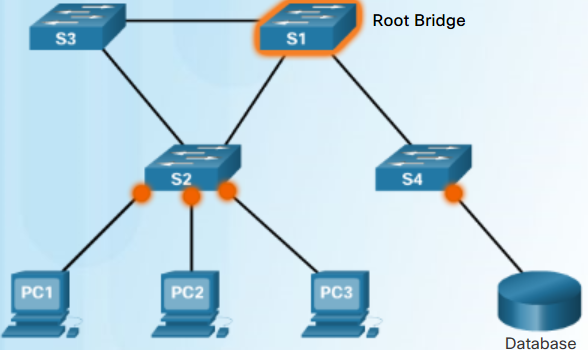
\includegraphics[ width=0.7\textwidth ]{pictures/EdgePort.PNG}
\end{figure}

\section{Configuration}

The default priority value of a switch is 32768. When an administrator wants a specific switch to become a root bridge, the bridge priority value must be adjusted to ensure it is lower than the bridge priority values of all the other switches on the network. By default, the priority for the root switch configured by \code{root primary} option is \textbf{24576}. The \code{root secondary} sets the priority of the switch to \textbf{28672}.

\begin{sexylisting}{STP}
spanning-tree mode pvst
spanning-tree vlan 10 root secondary
spanning-tree vlan 20 root primary

spanning-tree portfast default
spanning-tree portfast bpduguard default

interface F0/1
  spanning-tree portfast
  spanning-tree bpduguard enable
end

show spanning-tree
show spanning-tree vlan 10
show running-config interface f0/1
\end{sexylisting}

The command \code{spanning-tree vlan 10 priority 24576} can also be used to configure bridge priority. This command gives more granular control over the bridge priority value. Remember the priority value is configured in increments of 4,096 between 0 and 61,440. Cisco recommends caution when using this command. \\

The fourth command enables PortFast on all nontrunking interfaces, and the next command enables BPDU guard on all PortFast-enabled ports. 